\documentclass[a4paper, 11pt]{article}
\usepackage{graphicx}
\usepackage{url}
\usepackage{hyperref}
\usepackage[numbers]{natbib}
\usepackage{tabularx}
\usepackage{amsmath}
\usepackage{amssymb}
\usepackage{epstopdf}
\usepackage{inputenc}
\usepackage{geometry}
\usepackage{alphabeta}
\usepackage{float}
\usepackage{changepage}
\usepackage{lipsum}

\setlength{\oddsidemargin}{0mm}
\setlength{\evensidemargin}{-14mm}
\setlength{\marginparwidth}{0cm}
\setlength{\marginparsep}{0cm}
\setlength{\topmargin}{2mm}
\setlength{\headheight}{0mm}
\setlength{\headsep}{0cm}
\setlength{\textheight}{240mm}
\setlength{\textwidth}{168mm}
\setlength{\topskip}{0mm}
\setlength{\footskip}{10mm} 

\newcommand{\code}[1]{\texttt{#1}}
\newcommand{\refsec}[1]{\mbox{Section~\ref{sec:#1}}}
\newcommand{\refapp}[1]{\mbox{Appendix~\ref{sec:#1}}}
\newcommand{\refeqn}[1]{\mbox{(\ref{eqn:#1})}}
\newcommand{\reffig}[1]{\mbox{Figure~\ref{fig:#1}}}
\newcommand{\ud}{\mathrm{d}}                    % upright d (derivative)

\newcounter{foo}
\newcounter{bar}

\title{
    ENEL420 - Genetic Algorithms in Digital Signal Processing\\
    \vspace{1cm}
    \begin{large} 
        Department of Electrical and Computer Engineering\\
        University of Canterbury\\
    \end{large}
    \vspace{1cm}
}

\author{
    \small {Luke Trenberth (ID: 47277086)}\\
    \small {Hassan Alhujhoj (ID: 35352633)}\\
    }
\vspace{2cm}

\date{\small\today}
\begin{document}
\maketitle

\begin{abstract}
    I would like to say some bullshit here that summaries my report in an interesting way.
\end{abstract}

\pagebreak
\pagenumbering{roman}
\tableofcontents
\pagenumbering{arabic}
\pagebreak

\section{Introduction}\label{sec:intro}
    Genetic Algorithms are inspired by the mechanism of natural selection where the strongest and fittest
    individuals would likely be the winners in a competing environment. Genetic Algorithm is used as a direct 
    analogy of such natural evolution where it presumes that a potential solution of a problem is an individual 
    and can be represented by a set of parameters. These sets of parameters are regarded as the genes of a chromosome 
    and can be structured by a string of values in binary form. A fitness value is used to reflect the degree of 
    goodness of the chromosome for the problem which would be highly related with its objective value \cite{Man1997}.
    \\\\
    History has shown that the fitter chromosome tends to yield good quality offspring which means a
    better solution to the problem. Practically, a population pool of chromosomes must be randomly set initially. 
    The size of this population varies from one problem to the other. Each cycle of genetic operation is termed as 
    an evolving process where a subsequent generation is created from the chromosomes in the current population.  
    This evolving process can only be succeeded if a group of those chromosomes, which are generally called
    “parents” or a collection term “mating pool” are selected. The genes of the parents are then mixed to produce 
    offspring in the next generation. From this manipulation of genes process, the “better” chromosome will create a 
    larger number of offspring, and thus has a higher chance of survival in the subsequent generation, emulating the 
    survival-of-the-fittest mechanism in nature \cite{Man1997}.
    \\\\
    To make sure the desired termination criterion is reached, the cycle of evolution is repeated. The offspring of 
    the previous generation are reinserted into the model, further yielding higher quality offsprings \cite{Man1997}.
    \\\\
    There are two fundamental operators that facilitate the evolution cycle: Crossover and Mutation. Both operators 
    are required for such a process even though the selection routine. To further illustrate the crossover procedure, 
    the one-point crossover mechanism is shown in Figure \ref{Fig:crossover}. Genes are exchanged between parents to form 
    offspring. Mutations are randomly generated after crossover with a small probability of occurrence.
    
    \begin{figure}[h!]
        \centering
        \graphicspath{{./wiki/}}
        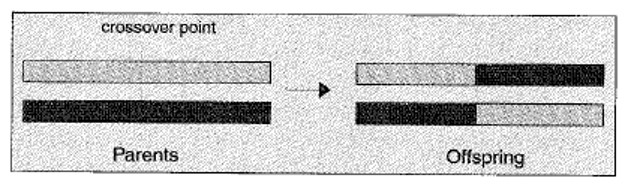
\includegraphics[scale=0.7]{crossover.png}
        \caption{Interference frequencies present in the ECG signal.}
        \label{Fig:crossover}
    \end{figure}

\section{Background}\label{sec:bg}
    \subsection{Digital Signal Processing of ECG Signals}\label{sec:bg_sub1}
        In assignment one, a noisy ECG signal with 1024Hz sampling frequency was provided to be filtered. 
        The assignment required the implementation of a notch filter with either an FIR or IIR filter.
        An FIR or IIR notch filter was suited to filter this ECG signal since there were a clear two 
        interference frequencies present within the frequency spectrum of the ECG signal.
        These interference frequencies were identified to be $f_{1} = 31.456Hz$ and $f_{2} = 74.36Hz$
        as shown in Figure \ref{Fig:rejFreq}. It should be noted that the first peak in Figure \ref{Fig:rejFreq} is the 
        DC component due to the use FFT to get the frequency response of the time domain ECG signal.
        
        \begin{figure}[h!]
            \centering
            \graphicspath{{./wiki/}}
            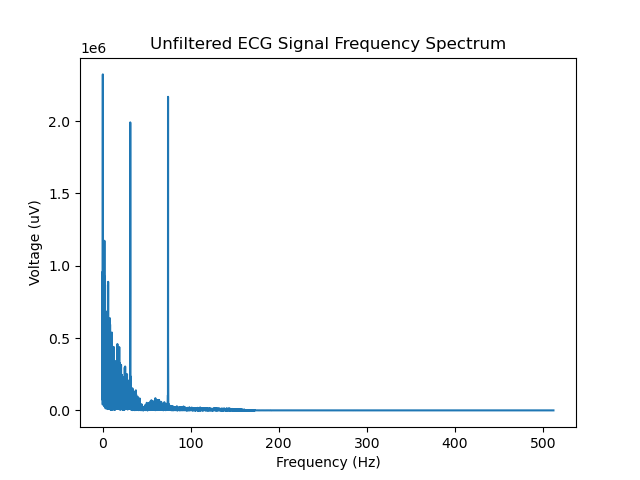
\includegraphics[scale=0.6]{ECG_freq_spectrum.png}
            \caption{Interference frequencies present in the ECG signal.}
            \label{Fig:rejFreq}
        \end{figure}

        One method to filter these two frequencies was to reject them with either a window or Parks-McClellan filters.
        
    \subsection{Genetic Algorithms}\label{sec:bg_sub2}
        Plz write something here.

\section{Method}\label{sec:meth}
    Describe the method followed for this assignment.
    \subsection{Creating a Population from DSP Singal Data}\label{sec:meth_sub1}
        Plz write something here.
    \subsection{Fitness Function}\label{sec:meth_sub2}
        Plz write something here.
    \subsection{Selecting Paranets for next GA Generations}\label{sec:meth_sub3}
        Plz write something here.
    \subsection{GA Operators}\label{sec:meth_sub4}
        Plz write something here.
        \subsubsection{Crossover}
            Crossover is a GA operator which is a recombination operator that comibines subparts of two paernt 
            chromosomes to produce offsprings that contain some parts of both parents' genetic material. Crossover
            is considered by 
        \subsubsection{Mutation}
            Plz write something here.
        \subsubsection{Parents}
            Plz write something here.
    \subsection{Filtering of ECG Signal Using FIR Filters}\label{sec:meth_sub5}
        \subsubsection{Window Filter}
            Plz write something here.
        \subsubsection{Parks-McClellan Filter}
            Plz write something here.

\section{Results}\label{sec:res}
    Describe\ae the results you've got. Don't give your opinion in here that goes in the Discussion.
    Unless combine the Results and Discussion sections \begin{equation} V = IR\end{equation}

    \subsection{Creating a Population from DSP Singal Data}\label{sec:meth_sub1}
    Plz write something here.
    \subsection{Fitness Function}\label{sec:meth_sub2}
    Plz write something here.
    \subsection{Selecting Paranets for next GA Generations}\label{sec:meth_sub3}
    Plz write something here.
    \subsection{GA Operators}\label{sec:meth_sub4}
    Plz write something here.
        \subsubsection{Crossover}
            Plz write something here.
        \subsubsection{Mutation}
            Plz write something here.
        \subsubsection{Parents}
            Plz write something here.
    \subsection{Filtering of ECG Signal Using FIR Filters}\label{sec:meth_sub5}
        \subsubsection{Window Filter}
            Plz write something here.
        \subsubsection{Parks-McClellan Filter}
            Plz write something here.
    
    \begin{figure}[h]
        \centering
        \graphicspath{{./wiki/}}
        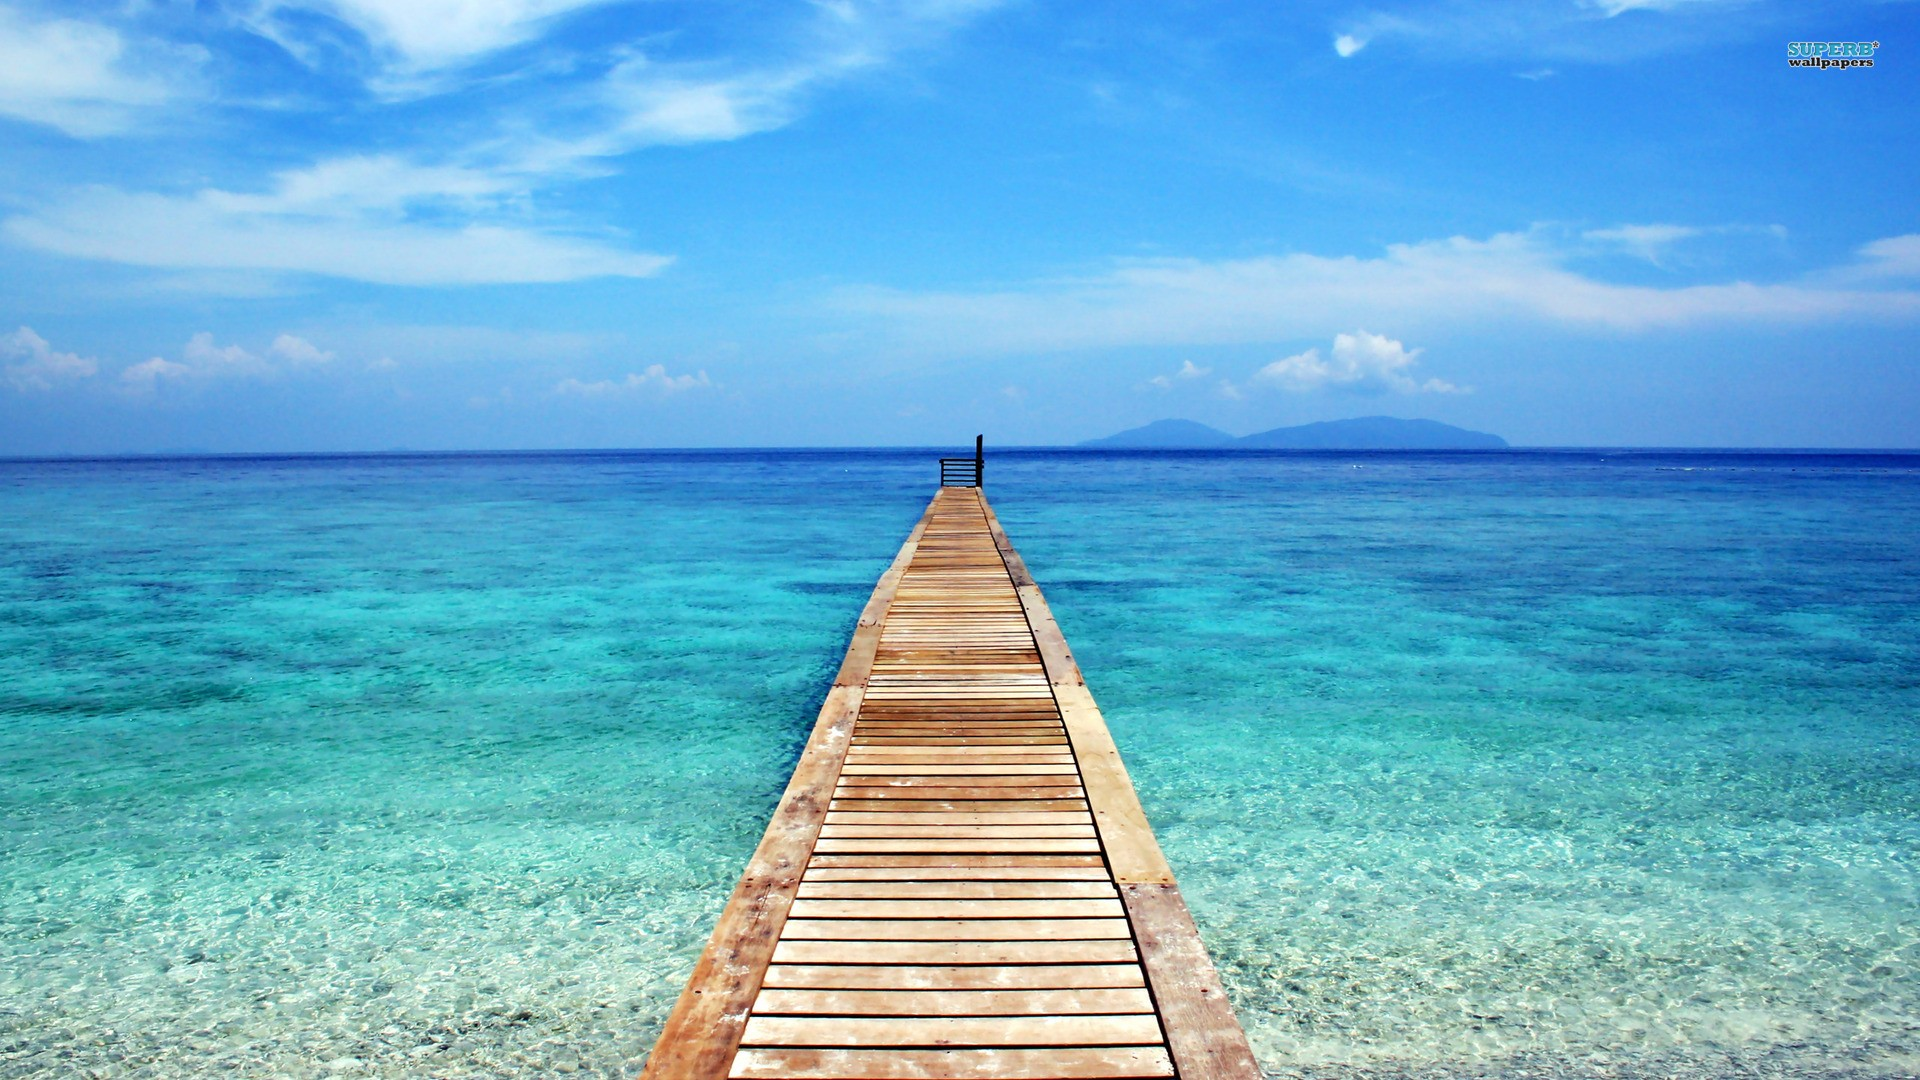
\includegraphics[scale=0.1]{fig.png}
        \caption{Shows that you can relax at this beautiful beach}
        \label{Fig:my_label}
    \end{figure}

\section{Discussion}\label{sec:dis}
    Discussion.

\section{Conclusion}\label{sec:conc}
    Reinstate the stuff you've talked about in the report. Don't introduce new materials in here.

\pagebreak
\bibliographystyle{IEEEtran}
\renewcommand{\bibname}{References}
\renewcommand{\bibsection}{\section{\bibname}}
\renewcommand{\cite}{\citep}
\bibliography{ref}
\pagebreak

\section{Appendices}
    \subsection{Appendix A}

\end{document}

